\section{Ergebnisse}

Um das Routing-Profil für Einsatzfahrzeuge auf seine Funktionalität zu validieren, müssen zwei unterschiedliche Aspekte beleuchtet werden.
Durch die Implementierung waren Veränderungen zum einen bei der Prozessierung des Graphen und zum anderen in den Routing-Ergebnissen zu erwarten.
Der Graph beziehungsweise das Straßennetzwerk und die Integration der Attribute für Feuerwehreinfahrten, Rad- und Fußwegen sowie Einbahnstraßen, musste bestätigt werden.
Außerdem wurden die Routing-Antworten auf ihre Praxistauglichkeit geprüft und daher die benötigten Fahrzeiten als auch die zurückgelegten Distanzen anhand von Testfahrten analysiert.


\subsection{Validierung des Graphen}

Für die folgenden Validierungen wurde ein Gebiet um Heidelberg als Datengrundlage verwendet.
Da der \gls{ors} zur Darstellung mehrerer Routen bisher noch nicht geeignet ist, wurden die Antworten im GeoJson Format mit der Website \textit{http://geojson.io} visualisiert.

\begin{figure}[htb]
\centering
\begin{subfigure}{0.49\textwidth}
\centering
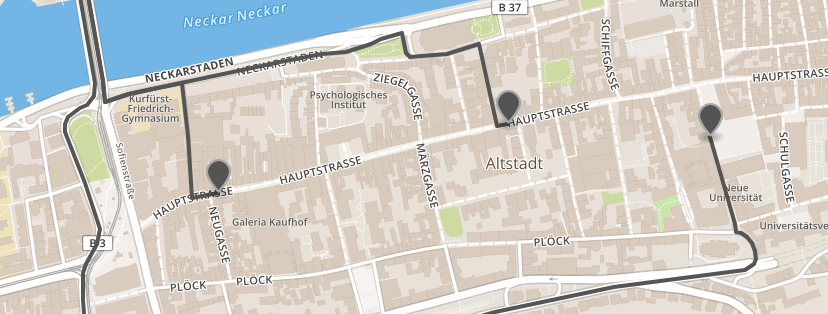
\includegraphics[width = 0.95\textwidth]{../media/Altstadt_emergency.png} \\
\caption{Löschfahrzeug Routing}
\label{fig:alteme}
\end{subfigure}
\begin{subfigure}{0.49\textwidth}
\centering
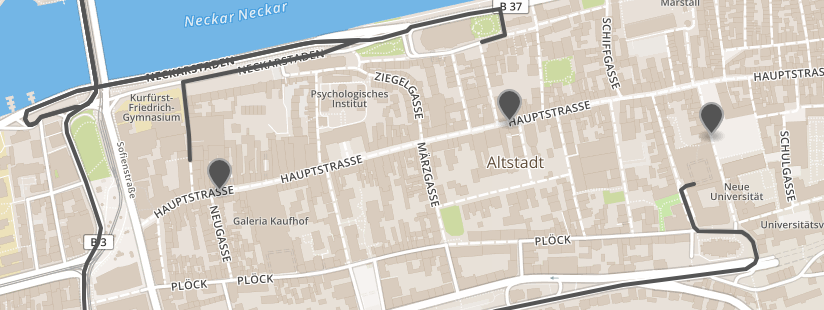
\includegraphics[width = 0.95\textwidth]{../media/Altstadt_car.png} \\
\caption{Auto Routing}
\label{fig:altcar}
\end{subfigure}
\caption[Routing in die Fußgängerzone der Heidelberger Altstadt]
{\centering Routing in die Fußgängerzone der Heidelberger Altstadt
\par\justifying\scriptsize
Straßensegmente die in OSM als Fußwege oder Fußgängerzonen getaggt sind, können von dem Profil für Löschfahrzeuge befahren werden.
Das Profil (a) steuert die Fußgängerzone von den Seitenstraßen an.
Dem Auto Profil ist es nicht erlaubt diesen Straßentyp zu benutzen, weshalb die Route vorzeitig endet (b).
}
\label{fig:footway}
\end{figure}

\subsubsection{Fußgängerzonen}

Die Verwendung neuer Wegtypen konnte eingebunden werden, wie in Abbildung~\ref{fig:footway} zu erkennen ist.
Hier wurden als Zielpunkte verschiedene Stellen auf der Fußgängerzone (v.a. Hauptstraße) in der Heidelberger Altstadt gewählt.
Im Gegensatz zu dem gewöhnlichen Auto-Profil des \gls{ors} findet das Profil für Einsatzfahrzeuge seinen Weg bis zum gewünschten Zielpunkt durch Fußgängerzonen.
Durch die niedrige Geschwindigkeitsangabe des Backends wird allerdings nicht durchgehend in der Fußgängerzone gefahren, welches zu manchen Nachtzeiten durchaus schneller erfolgen kann.
Stattdessen werden die Zielpunkte von den schnelleren Seitenstraßen aus angefahren.

\begin{figure}[H]
\centering
\begin{subfigure}{0.49\textwidth}
\centering
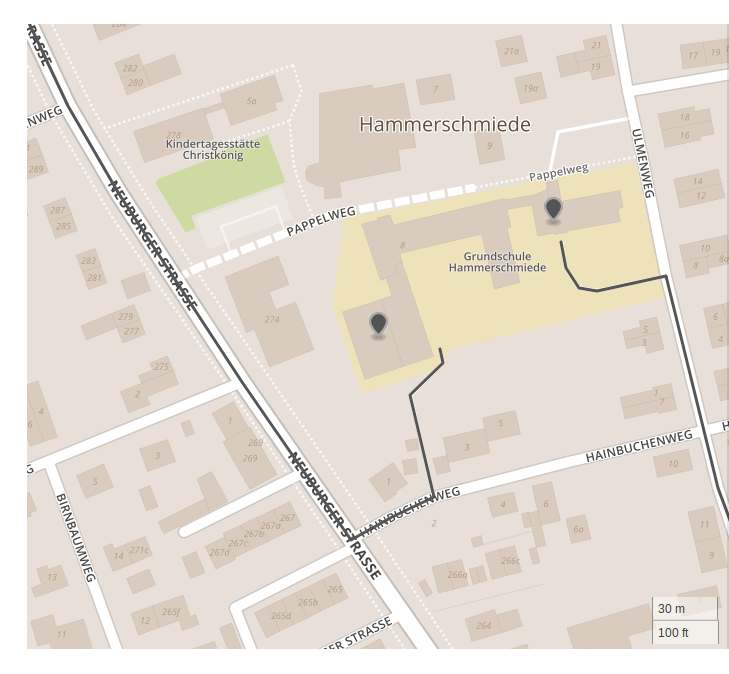
\includegraphics[width = 0.95\textwidth]{../media/schoolfire.png} \\
\caption{Löschfahrzeug Routing}
\label{fig:schoolfire}
\end{subfigure}
\begin{subfigure}{0.49\textwidth}
\centering
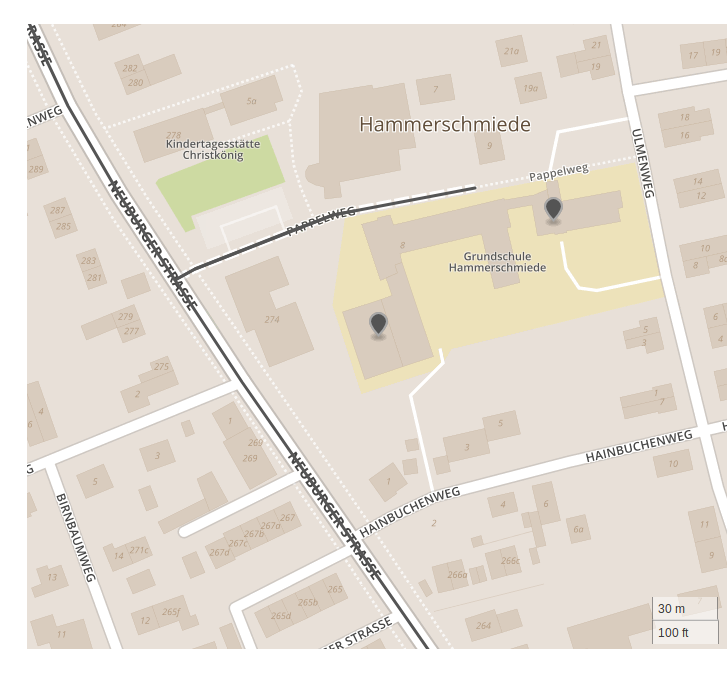
\includegraphics[width = 0.95\textwidth]{../media/schoolcar.png} \\
\caption{Auto Routing}
\label{fig:schoolcar}
\end{subfigure}
\caption[Routing durch Feuerwehreinfahrten]
{\centering Routing durch Feuerwehreinfahrten
\par\justifying\scriptsize
Straßensegmente die in OSM als Notfalleinfahrt gekennzeichnet sind, können von dem Profil für Löschfahrzeuge befahren werden.
Das Profil (a) erreicht das Schulgebäude über die vorgesehenen Wege während das Auto Profil (b) seine Anfahrt auf der Gebäuderückseite beendet.
}
\label{fig:school}
\end{figure}

\subsubsection{Notfalleinfahrten}


Auch die Nutzung von Notfalleinfahrten konnte implementiert werden.
Abbildung~\ref{fig:school} zeigt zwei Zielpunkte, die sich auf dem Gebäude einer Grundschule in Augsburg befinden. 
Während das Einsatzfahrzeug-Profil die verfügbaren Feuerwehreinfahrten benutzt (Abb.~\ref{fig:schoolfire}), kann mit gewöhnlicher Routenführung nur die Rückseite des Schulgebäudes erreicht werden (Abb.~\ref{fig:schoolcar}).

\begin{figure}[htb]
\centering
\begin{subfigure}{0.49\textwidth}
\centering
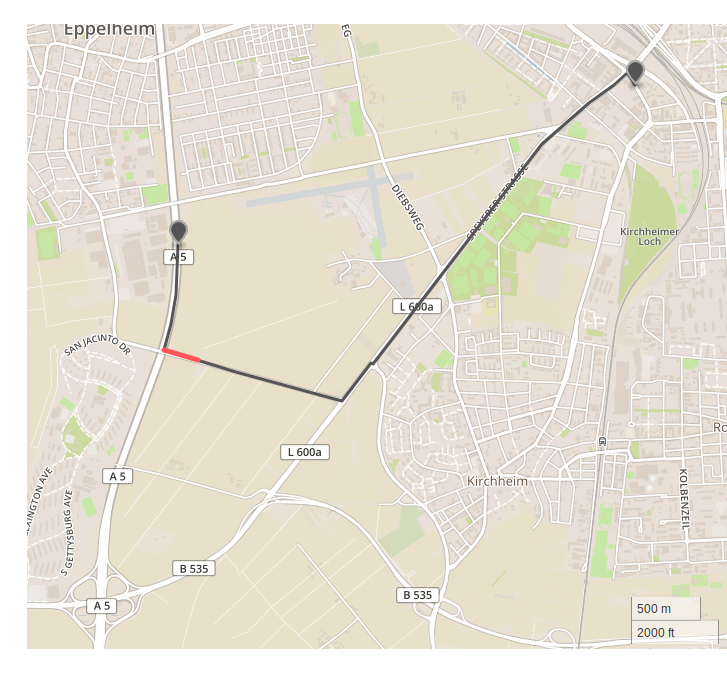
\includegraphics[width = 0.95\textwidth]{../media/notauffahrt.png} \\
\caption{Löschfahrzeug Routing}
\label{fig:emeramp}
\end{subfigure}
\begin{subfigure}{0.49\textwidth}
\centering
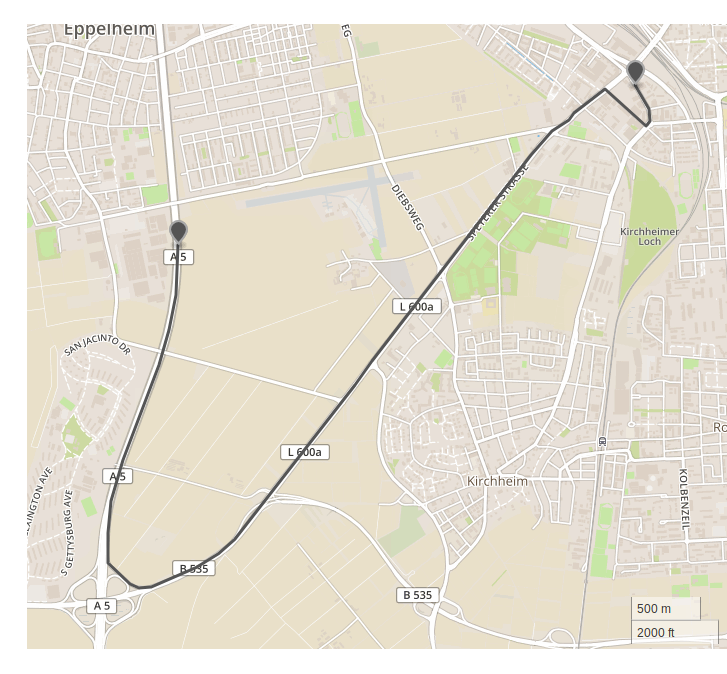
\includegraphics[width = 0.95\textwidth]{../media/normalauffahrt.png} \\
\caption{Auto Routing}
\label{fig:normalramp}
\end{subfigure}
\caption[Routing auf die $A5$ über eine Notauffahrt]
{\centering Routing auf die $A5$ über eine Notauffahrt
\par\justifying\scriptsize
In diesem Beispiel ist die Anfahrt der $A5$ von Heidelberg aus zu sehen. Das Löschfahrzeug-Profil (a) kann durch die Nutzung der Notauffahrt (rote Linie) gegenüber dem Auto-Profil (b) mehrere Kilometer einsparen.
}
\label{fig:ramp}
\end{figure}

In einem weiteren Beispiel wird die schnellste Route zu einem Punkt auf der $A5$ auf der östlichen Spur südlich von Eppelheim in Heidelberg mit Startpunkt in der Weststadt gesucht (Abb.~\ref{fig:ramp}).
Für den normalen Verkehr führt der Weg über das südliche Autobahnkreuz (Abb.~\ref{fig:normalramp}).
Ein Einsatzfahrzeug kann stattdessen vorher auf eine Nebenstraße einbiegen und die in Abbildung~\ref{fig:emeramp} rot eingefärbte Notauffahrt verwenden.
Damit kann in diesem Fall eine Strecke von mehr als 2,5 Kilometern eingespart werden.

\begin{figure}[H]
\centering
\begin{subfigure}{0.49\textwidth}
\centering
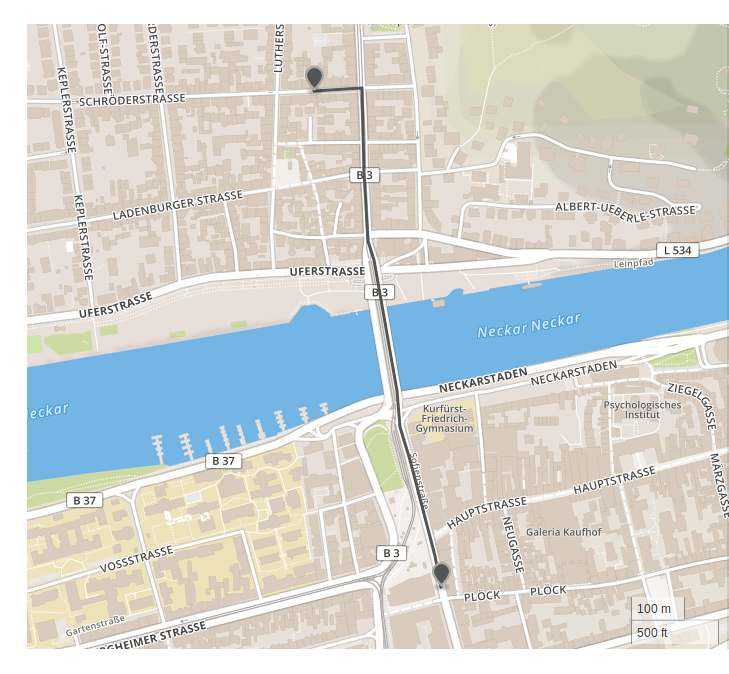
\includegraphics[width = 0.95\textwidth]{../media/onewayeme.png} \\
\caption{Löschfahrzeug Routing}
\label{fig:onewayeme}
\end{subfigure}
\begin{subfigure}{0.49\textwidth}
\centering
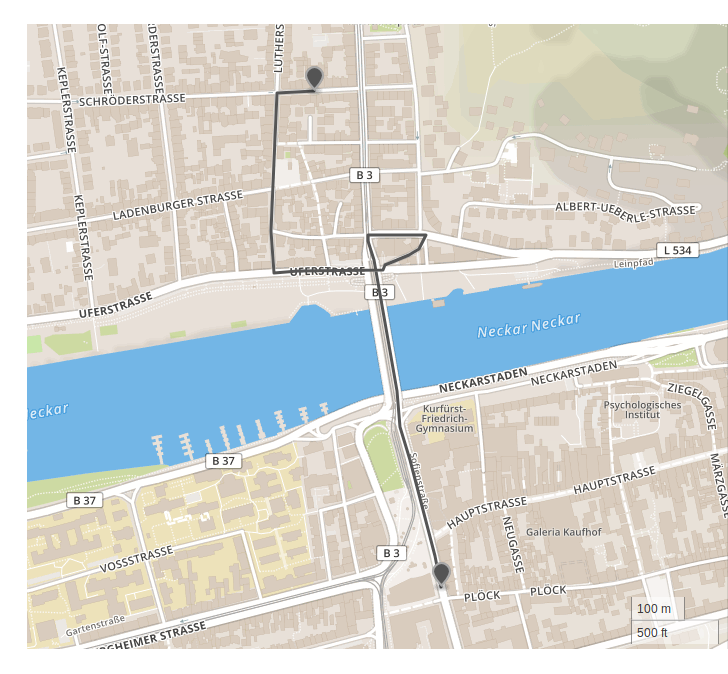
\includegraphics[width = 0.95\textwidth]{../media/onewaycar.png} \\
\caption{Auto Routing}
\label{fig:onewaycar}
\end{subfigure}
\caption[Routing durch Einbahnstraßen]
{\centering Routing durch Einbahnstraßen
\par\justifying\scriptsize
Um zu einem Zielpunkt in Neuenheim zu gelangen, kann das Profil für Löschfahrzeuge eine einfache Route wählen und eine Einbahnstraße, kurz vor dem Ziel, entgegen der Fahrtrichtung verwenden (a).
Das Auto-Profil muss Einbahnstraßen beachten und daher einen Umweg zum Ziel wählen (b).
}
\label{fig:oneway}
\end{figure}

\subsubsection{Einbahnstraßen}

Die Verwendung von Einbahnstraßen in Gegenrichtung konnte ebenfalls bestätigt werden.
Auch durch diese Funktion können kürzere Wegstrecken für die Einsatzfahrzeuge gefunden werden. 
Durch die große Zahl von Einbahnstraßen in Heidelberg-Neuenheim kann das Profil für Einsatzfahrzeuge (Abb.~\ref{fig:onewayeme}) gegenüber dem Auto-Profil (Abb.~\ref{fig:oneway}) eine wesentlich passendere Route nutzen und muss auf diese Weise etwa 400 Meter weniger zurücklegen.

\begin{figure}[H]
\centering
\begin{subfigure}{0.49\textwidth}
\centering
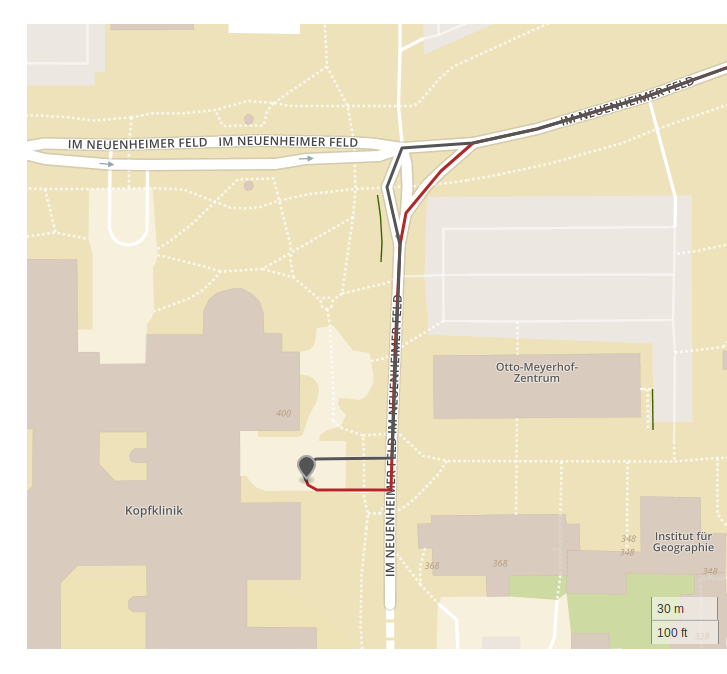
\includegraphics[width = 0.95\textwidth]{../media/oppositecurve.png} \\
\caption{Abkürzung in Kurven}
\label{fig:oppositecurve}
\end{subfigure}
\begin{subfigure}{0.49\textwidth}
\centering
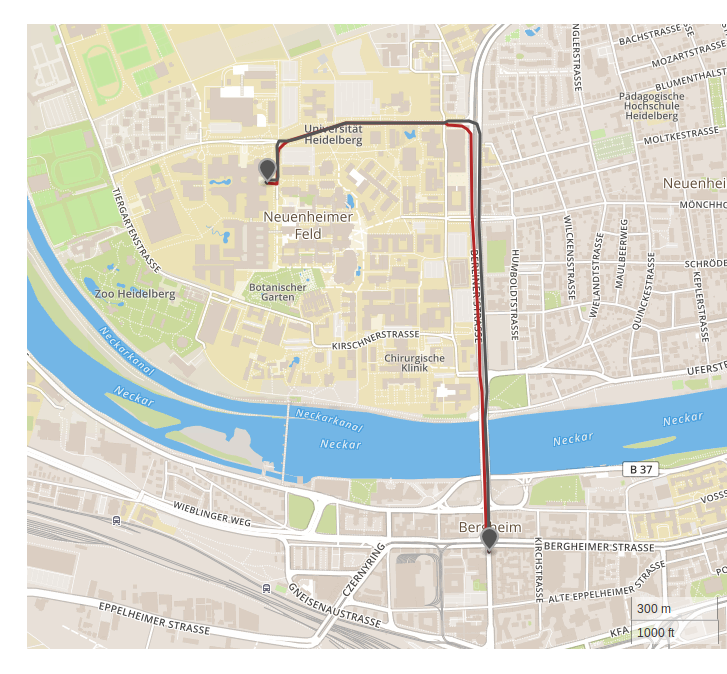
\includegraphics[width = 0.95\textwidth]{../media/oppositelane.png} \\
\caption{Dauerhafte Nutzung der Gegenfahrbahn}
\label{fig:oppositelane}
\end{subfigure}
\begin{subfigure}{0.90\textwidth}
\centering
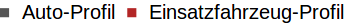
\includegraphics[width = 0.45\textwidth]{../media/legend4.png} \\
\end{subfigure}
\caption[Routing auf der Gegenfahrbahn]
{\centering Routing auf der Gegenfahrbahn
\par\justifying\scriptsize
Durch die uneingeschränkte Verwendung von Einbahnstraßen routet das Löschfahrzeug-Profil oft über lange Strecken auf der Gegenfahrbahn. Auch an Abbiegungen wird die Spur des Gegenverkehrs verwendet.
}
\label{fig:opposite}
\end{figure}

Allerdings verwendet das Löschfahrzeug-Profil Einbahnstraßen bisher ohne Einschränkung.
Daher wird die Gegenfahrbahn auch bei einem Gewinn von wenigen Sekunden verwendet (Abb.~\ref{fig:opposite}).
Deswegen wird, wie Abbildung~\ref{fig:oppositelane} zeigt, über weite Strecken die Gegenfahrbahn verwendet, obwohl unmittelbar daneben auch die normale Spur verfügbar ist.
Außerdem wird an größeren Kreuzungen die Abbiegespur des Gegenverkehrs verwendet, was keine realistische Lösung darstellt (Abb.~\ref{fig:oppositecurve}).

\newpage
\subsection{Validierung der Distanzen und der Fahrzeit}

Im Folgenden wurden Isochronen mit der Freiwilligen Feuerwehr Gablingen als Zentrum berechnet (\texttt{48.454063,10.824415 [Latitude, Longitude]}).
Folgende Einstellungen wurden dabei genutzt:
\sloppy
\begin{itemize}
\item Distanz: 5 Minuten
\item Intervall: 1 Minuten
\item Maximale Geschwindigkeit: 80 km/h für Löschfahrzeug sowie Heavy-Vehicle; 130 km/h für PKW sowie Einsatzfahrzeug
\item Heavy-Vehicle-Einstellungen für Löschfahrzeug- und Heavy-Vehicle-Profil: Länge=7m ; Breite= 2.5m; Höhe= 3m; Gewicht= 7.5t
\end{itemize}
\fussy

Die ersten Ergebnisse lieferten zu erwartende Resultate (Abb.~\ref{fig:isochrones}), denn das Profil für allgemeine Einsatzfahrzeuge (Abb.~\ref{fig:isoeme}) konnte gegenüber dem normalen Auto-Profil (Abb.~\ref{fig:isocar}) einen größeren Bereich abdecken.
Genauso ist das in fünf Minuten zu erreichende Gebiet für Löschfahrzeuge (Abb.~\ref{fig:isofire}) sichtbar größer als für das Heavy-Vehicle-Profil (Abb.~\ref{fig:isohgv}).
Auffällig sind dabei die ausgedehnten 5-Minuten-Isochronen, welche durch den Alpha-Shape Algorithmus (Kapitel \ref{sec:form}) auch unzugängliche Bereiche beinhalten.

Nach einer Testfahrt der \gls{ffl} wurde allerdings ersichtlich, dass die Ergebnisse nicht im realistischen Bereich liegen.
In fünf Minuten konnte das Löschfahrzeug auf der Einsatzfahrt vom Startpunkt in Gablingen Richtung Muttershofen nur den nordwestlichen Rand von Lützelburg erreichen.
Das Profil des Löschfahrzeugs erreichte allerdings Orte über Muttershofen hinaus.

\begin{figure}[H]
\centering
\begin{subfigure}{0.49\textwidth}
\centering
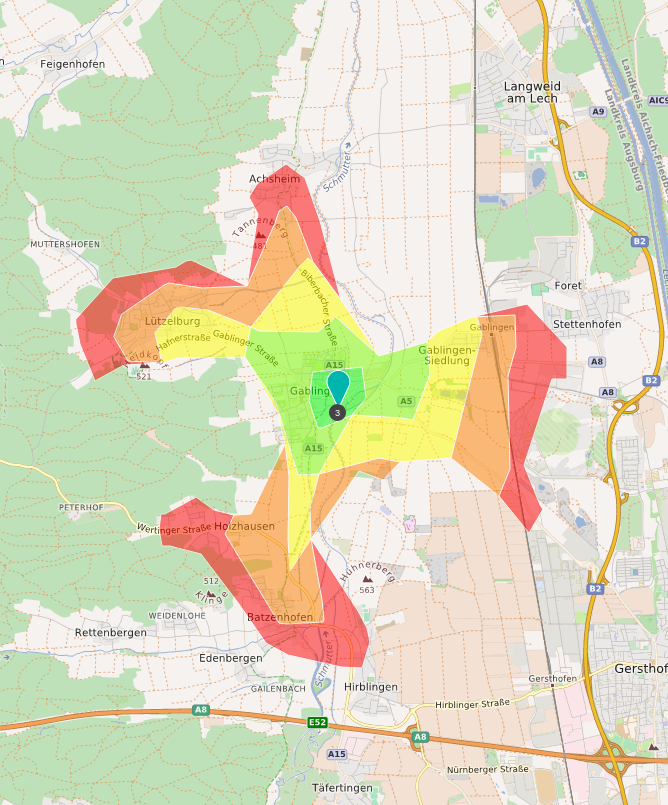
\includegraphics[width = 0.75\textwidth]{../media/isohgv.png} \\
\caption{Heavy-Vehicle-Profil}
\label{fig:isohgv}
\end{subfigure}
\begin{subfigure}{0.49\textwidth}
\centering
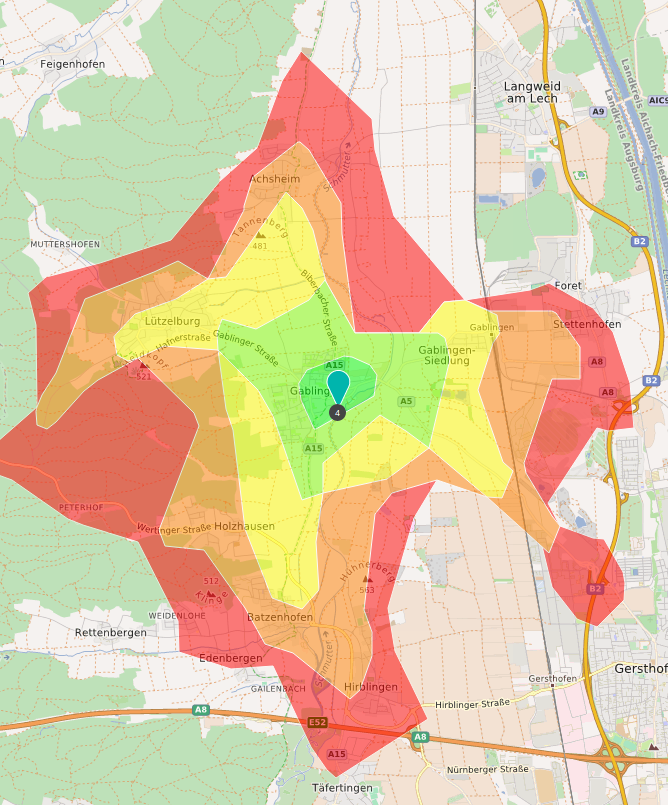
\includegraphics[width = 0.75\textwidth]{../media/isocar.png} \\
\caption{Auto-Profil}
\label{fig:isocar}
\end{subfigure}
\begin{subfigure}{0.49\textwidth}
\centering
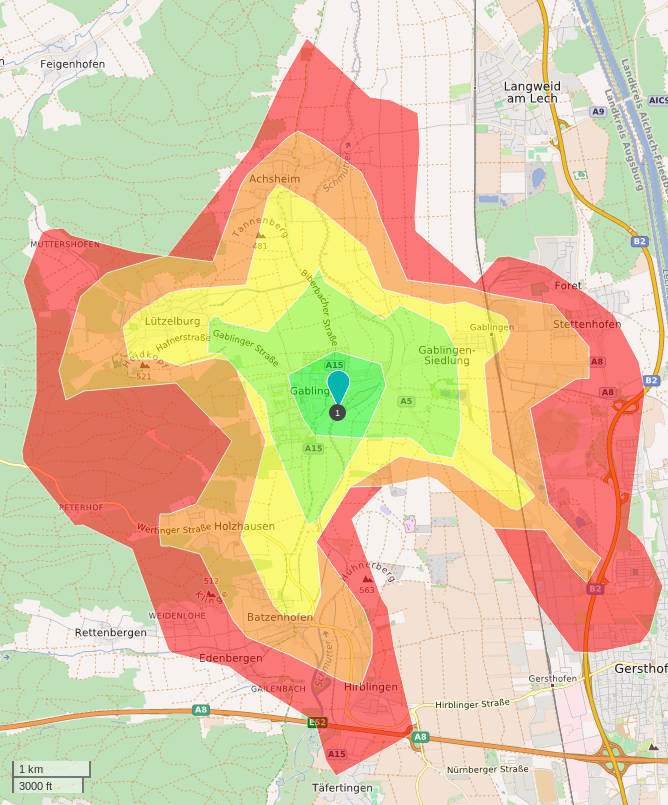
\includegraphics[width = 0.75\textwidth]{../media/isofire.png} \\
\caption{Löschfahrzeug-Profil}
\label{fig:isofire}
\end{subfigure}
\begin{subfigure}{0.49\textwidth}
\centering
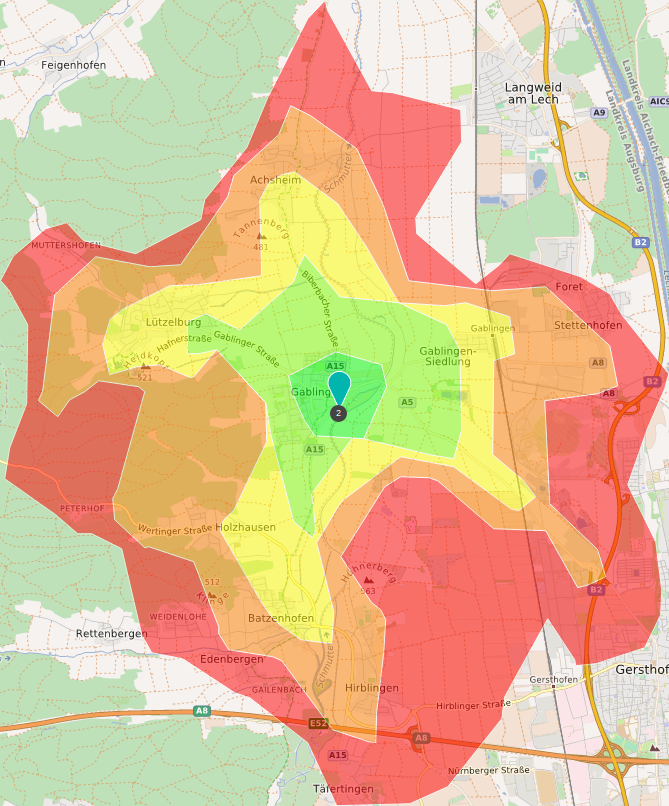
\includegraphics[width = 0.75\textwidth]{../media/isoeme.png} \\
\caption{allg. Einsatzfahrzeug-Profil}
\label{fig:isoeme}
\end{subfigure}
\begin{subfigure}{0.90\textwidth}
\centering
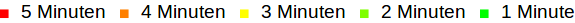
\includegraphics[width = 0.75\textwidth]{../media/legendiso.png} \\
\end{subfigure}
\caption[Ergebnis Isochronen]
{\centering Ergebnis Isochronen
\par\justifying\scriptsize
Die Abbildung zeigt die Isochronen für 1-5 Minuten für die Profile: Heavy-Vehicle (a), Auto (b), Löschfahrzeug (c) und allgemeines Einsatzfahrzeug (d).
Durch die höheren Geschwindigkeiten und die zusätzlichen Wegtypen decken die Isochronen der Einsatzfahrzeuge größere Gebiete ab.
}
\label{fig:isochrones}
\end{figure}

Um genaue Anpassungen am Backend vorzunehmen, wurde zunächst eine weitere Testfahrt durchgeführt, bei der für jede volle Minute der Aufenthaltsort des Fahrzeuges markiert wurde (Abb.~\ref{fig:drive1}).
Diese Angaben wurden mit den bisherigen Rückgabewerten des Profils verglichen.
Wie aus der Gesamtdauer für die Strecke in Tabelle \ref{tab:driveinit} ersichtlich wird, ist das Profil für Einsatzfahrzeuge ungefähr 90 Sekunden zu schnell.

\begin{figure}[H]
\centering
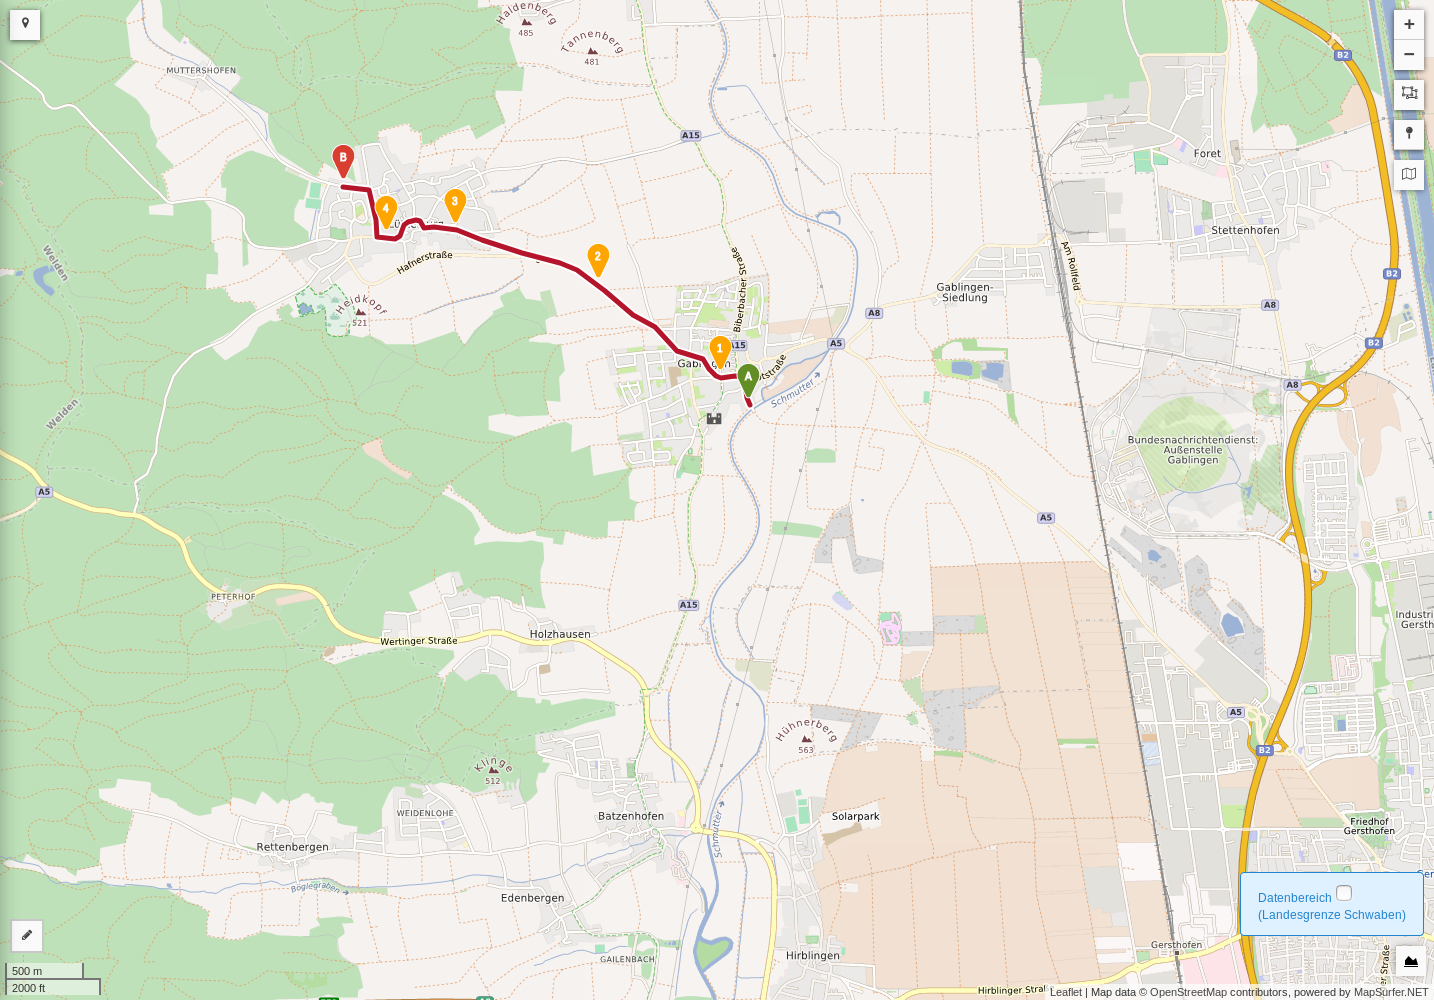
\includegraphics[width = 0.7 \textwidth]{../media/Fahrt1.png} \\
\caption[Teststrecke 1]
{\centering Teststrecke 1
\par\justifying\scriptsize
Die erste Testfahrt wurde von dem Feuerwehrstützpunkt (A) in Gablingen aus in Richtung Lützelburg durchgeführt.
Nach jeder vollen Minute wurde die Position registriert und als Marker auf der Route platziert ($B=5$).
}
\label{fig:drive1}
\end{figure}

\begin{table}[htb]
\centering
\small
\caption{Teststrecke 1 -- 1. Auswertung}
\label{tab:driveinit}
\begin{tabular}{|l|r|r|r|r|r|}
\hline
Wegpunkt                               & \multicolumn{1}{c|}{1} & \multicolumn{1}{c|}{2} & \multicolumn{1}{c|}{3} & \multicolumn{1}{c|}{4} & \multicolumn{1}{c|}{B}      \\ \hline
Distanz                                & 363,2$m$                & 1352,8$m$               & 2331,9$m$               & 2862,3$m$               & 3387,3$m$               \\ \hline
Fahrtzeit (Profil)                     & 28,6$s$                 & 88,7$s$                 & 139,4$s$                & 177,6$s$                & 209,8$s$                \\ \hline
Fahrtzeit (Fahrt 1)                  & 60,0$s$                 & 120,0$s$                & 180,0$s$                & 240,0$s$                & 300,0$s$                \\ \hline
Fahrtzeit Abschnitt                    & 28,6$s$                 & 60,1$s$                 & 50,7$s$                 & 38,2$s$                 & 32,2$s$                 \\ \hline
Fahrtzeit Abschnitt (Fahrt 1)        & 60,0$s$                 & 60,0$s$                 & 60,0$s$                 & 60,0$s$                 & 60,0$s$                 \\ \hline
Geschwindigkeit                        & 45,7$km/h$              & 59,3$km/h$              & 69,5$km/h$              & 50,0$km/h$              & 58,7$km/h$              \\ \hline
Geschwindigkeit (Fahrt 1)            & 21,8$km/h$              & 59,4$km/h$              & 58,7$km/h$              & 31,8$km/h$              & 31,5$km/h$              \\ \hline
\end{tabular}
\end{table}

Die große Differenz tritt aufgrund von fehlenden Beschleunigungs- und Bremszeiten auf.
Bisher wird bei der Berechnung der Fahrzeit lediglich 90$\%$ des für ein Segment vorgegebenen Geschwindigkeitslimits verwendet.
Damit soll sichergestellt sein, dass die Geschwindigkeitsbegrenzung definitiv eingehalten wird.
Dieser Faktor wurde allerdings für die Implementierung in dieser Arbeit entfernt.
Demnach wird ein Straßensegment auf dem 50 km/h gefahren werden dürfte über die komplette Distanz mit 50 km/h befahren.
In der Realität benötigt ein Fahrzeug dieser Größenordnung allerdings einige Sekunden um diese Geschwindigkeit aus dem Stand zu erreichen.
Der selbe Zusammenhang besteht für Bremsvorgänge ebenfalls.
Daraus gehen drei Szenarien hervor, welche nach festgelegter Route einen Einfluss auf die Fahrzeit haben können.
Das sind der Start, ein Abbiegevorgang (engl.: Turn) und die Ankunft.
Es gibt weitere Faktoren die beispielsweise andere Verkehrsteilnehmer betreffen, allerdings sind die drei genannten Szenarien aus jeder Routenführung ersichtlich und werden bei einer Einsatzfahrt in der Regel auftreten.

Anhand dieses Zusammenhangs wurde eine weitere Java-Klasse \texttt{AccelerationWeighting} in der die zusätzliche Zeit für diese Szenarien berechnet wird, implementiert (Siehe Anhang S.\pageref{sec:source}).
Diese Klasse soll zwei Funktionen erfüllen:
Zum einen muss bereits bei der Suche nach dem schnellsten Weg im Gegensatz zu geraden Strecken eine zusätzliche Zeit für Abbiegevorgänge mit einfließen.
Zum anderen müssen bei der Berechnung der Fahrzeit Start-, Ankunfts- und Abbiegezeit mit berücksichtigt werden.

\begin{table}[htb]
\centering
\caption{Teststrecke 1 -- Fahrzeit}
\label{tab:drive11}
\begin{tabular}{|l|r|r|}
\hline
Wegpunkt & Fahrtzeit & Differenz \\ \hline 
1$min$ & 78,3$s$ & $+18,3s$ \\
2$min$ & 138.5$s$ & $+18,5s$ \\
3$min$ & 188.5$s$ & $+8,5s$ \\
4$min$ & 226.7$s$ & $-3,3s$ \\
5$min$ & 298.9$s$ & $-1,1s$ \\
\hline
\end{tabular}
\end{table}

Es stellt sich nun die Frage, auf welche Art ein Abbiegevorgang auf dem Graphen identifiziert werden kann.
Die Änderung des Straßennamens ist sicherlich eine Möglichkeit viele Abbiegevorgänge abzudecken.
Allerdings ist nicht immer ein Straßenname vorhanden und nicht immer bedeutet der Wechsel des Straßennamens, dass in diese Straße eingebogen werden muss.
Eine effizientere Lösung bietet die Ausrichtung der Straßensegmente, da hier die Daten in allen Fälle vorhanden sind.
Deshalb wird in der AccelerationWeighting Klasse an Tower Nodes (Kreuzungen) der Winkel zwischen dem letzten und dem nächsten Straßensegment berechnet.
Eine Abbiegung bzw. eine enge Kurve wird in dieser Arbeit durch einen Winkel zwischen 50 und 140 Grad definiert.
Bei einer Routing-Abfrage wird in einem solchen Fall das Gewicht der auf die Kurve folgenden Kante erhöht.
Ebenso wird sobald der schnellste Weg ermittelt ist an diesen Stellen die Bremszeit vor der Abbiegung und die Beschleunigungszeit nach der Abbiegung zur Gesamtzeit des folgenden Wegsegmentes addiert.
Der gleiche Vorgang wird für Start und Ziel durchgeführt.
Die addierte Zeit wird als \textit{Penalty} (dt.: Strafe) bezeichnet.

\begin{figure}[H]
\centering
\caption[Teststrecke 2]
{\centering Teststrecke 2
\par\justifying\scriptsize
Die zweite Testfahrt wurde von dem Feuerwehrstützpunkt (A) in Gablingen aus in östliche Richtung durchgeführt.
Nach jeder vollen Minute wurde die Position registriert und als Marker auf der Route platziert ($B=5$).
}
\label{fig:drive2}
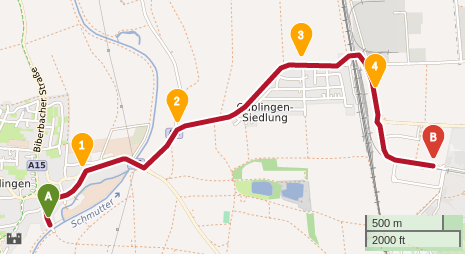
\includegraphics[width = 0.70 \textwidth]{../media/Fahrt2crop.png} \\
\end{figure}

Anhand der vorliegenden Testfahrt wurde das Profil derart kalibriert, dass durch die Penalties für Abbiegungen, Start und Ziel die fehlenden 90 Sekunden benötigt wurden.
Für Start sowie Ankunft wurden 15 und für Abbiegungen 20 Sekunden veranschlagt.

Mit dem neu eingestellten Profil wurde nun erneut eine Anfrage für die erste Testfahrt gesendet.
Wie erwartet, benötigte das Profil nun für diesen Weg ebenfalls fast genau fünf Minuten.
In Tabelle \ref{tab:drive11} ist die Differenz zu den einzelnen Minutenmarkern der 1. Testfahrt für diese Anfrage zu sehen.
Diese Ergebnisse zeigen dass das Profil den ersten Teil der Route zu langsam und den zweiten Teil zu schnell absolviert.

\begin{table}[htb]
\centering
\caption{Teststrecke 2 -- Fahrzeit}
\label{tab:drive2}
\begin{tabular}{|l|r|r|}
\hline
Wegpunkt & Fahrtzeit & Differenz \\ \hline 
1$min$ & 86.6$s$ & $+26.6s$ \\
2$min$ & 149.9$s$ & $+29.9s$ \\
3$min$ & 207.5$s$ & $+27.5s$ \\
4$min$ & 253.5$s$ & $+13.5s$ \\
5$min$ & 318.6$s$ & $+18.6s$ \\
\hline
\end{tabular}
\end{table}


Diese Kalibrierung wurde an zwei weiteren Testfahrten (Abb.~\ref{fig:drive2} und \ref{fig:drive3}) vom selben Ausgangspunkt überprüft.

In den Tabellen \ref{tab:drive2} und \ref{tab:drive3} ist zu sehen, das 8 von 10 Wegpunkten um mehr als 20 Sekunden, in 3 Fällen sogar 40 Sekunden zu spät erreicht werden.
Mit den Ergebnissen dieser Testfahrten steht fest: das Profil ist noch erheblich zu langsam und die Penalties zu hoch.

\begin{figure}[H]
\centering
\caption[Teststrecke 3]
{\centering Teststrecke 3
\par\justifying\scriptsize
Die dritte Testfahrt wurde von dem Feuerwehrstützpunkt (A) in Gablingen aus nach Holzhausen durchgeführt.
Nach jeder vollen Minute wurde die Position registriert und als Marker auf der Route platziert ($B=5$).
}
\label{fig:drive3}
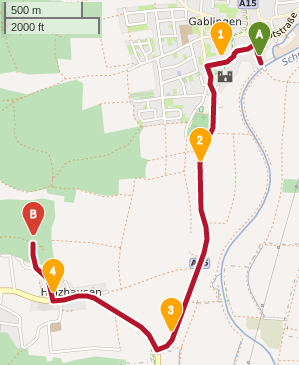
\includegraphics[width = 0.40 \textwidth]{../media/Fahrt3crop.png} \\
\end{figure}

\begin{table}[]
\centering
\caption{Teststrecke 3 -- Fahrzeit}
\label{tab:drive3}
\begin{tabular}{|l|r|r|}
\hline
Wegpunkt & Fahrtzeit & Differenz \\ \hline 
1$min$ &  89.8$s$ & $+29.8s$ \\
2$min$ &  162.4$s$ & $+42.4s$ \\
3$min$ &  213$s$ & $+33s$ \\
4$min$ &  282.3$s$ & $+42.3s$ \\
5$min$ &  343.9$s$ & $+43.9s$ \\
\hline
\end{tabular}
\end{table}

Die Penalties für Start und Ankunft wurden für die folgenden Analysen um die Hälfte reduziert und lagen somit bei 7,5 Sekunden.
Penalties für Abbiegungen wurden auf 16 Sekunden reduziert.

Mit der neuen Gewichtung wurden die Anfragen für die drei Testfahrten erneut gesendet und mit den Minuten-Markierungen der wirklich benötigten Zeiten verglichen.
Die Ergebnisse sind der Tabelle \ref{tab:all} zu entnehmen.

\begin{table}[htb]
\centering
\caption{2. Auswertung der drei Testfahrten}
\label{tab:all}
\begin{tabular}{|l|r|r|r|r|r|r|}
\hhline{~|-|-|-|-|-|-}
\multicolumn{1}{l|}{} & \multicolumn{2}{c|}{Fahrt 1} & \multicolumn{2}{c|}{Fahrt 2} & \multicolumn{2}{c|}{Fahrt 3} \\ \hline
Wegpunkt              & Fahrtzeit   & Differenz     & Fahrtzeit   & Differenz     & Fahrtzeit  & Differenz      \\ \hline 
1$min$                & 59.5$s$     & -0.5$s$        & 67.6$s$     & +7.6$s$        & 70.8$s$    & +10.8$s$        \\
2$min$                & 119.5$s$    & -0.5$s$        & 126.9$s$    & +6.9$s$        & 139.4$s$   & +19.4$s$        \\
3$min$                & 169.5$s$    & -10.5$s$       & 184.5$s$    & +4.5$s$        & 190$s$     & +10$s$          \\
4$min$                & 207.7$s$    & -32.2$s$       & 230.5$s$    & -10.5$s$       & 255.2$s$   & +15.2$s$        \\
5$min$                & 271.9$s$    & -28.1$s$       & 291.6$s$    & -8.4$s$        & 312.9$s$   & +12.9$s$        \\
\hline
\end{tabular}
\end{table}


Um die Testfahrten genauer analysieren zu können, wurde das Backend um bisher fehlende Funktionen für die Rückgabe von zusätzlichen Informationen erweitert.
Dabei wurden die Speicherobjekte für Wegtypen und Wegoberfläche hinzugefügt und zusätzlich die Höheninformationen der Punkte zurückgegeben.
Im Frontend konnten dadurch nun die Wegtypen und Wegoberflächen aber auch die Steigung und somit auch ein Höhenprofil angezeigt werden.
Außerdem wurde ein Feature zur Darstellung der Höchstgeschwindigkeit der einzelnen Streckensegmente eingebaut.